% !TEX program = lualatex
% NOTE: iac.cls uses fontspec/TeX Gyre Termes, so this file must be compiled
% with LuaLaTeX or XeLaTeX -- pdfLaTeX aborts with a fatal fontspec error.
\documentclass{iac}

% hyperref is ALREADY loaded by iac.cls (with colorlinks=false, allcolors=blue).
% Do not load it again: \usepackage{hyperref} here would give an option clash,
% and inside the document body it is illegal ("can be used only in preamble").
% Change its behaviour with \hypersetup in the preamble instead.
\usepackage{graphicx}
\usepackage{floatflt}
\usepackage{array}
\usepackage{tikz}
\usetikzlibrary{calc}
\usepackage{pgfplots}
\usepackage{subcaption}
\usepackage{xcolor}
\usepackage{tablefootnote}
\usepackage{float}
\usepackage{orcidlink}
\usepackage{pgfplots}
\usepackage{booktabs}     % For professional \toprule, \midrule, \bottomrule
\usepackage{tabularx}     % For adjustable-width wrapping columns (X type)
\usepackage{threeparttable} % For clean, automated table footnotes
\hypersetup{
    colorlinks=true,       % true = colored text; false = boxed links
    linkcolor=cyan,         % Color of internal links (sections, figs)
    citecolor=cyan,       % Color of citations
    filecolor=cyan,     % Color of file links
    urlcolor=cyan,         % Color of external URLs
    pdftitle={SWaP-Optimized Hyperspectral Payload Architecture for AI-Driven Precision Agriculture Missions in LEO Small Satellites},
    pdfauthor={Haruna H. Mohammed, Dinaol Gadisa, Hyochoong Bang}
}

\addbibresource{references.bib}

\begin{document}

\IACconference{77}
\IAClocation{Antalya, Türkiye}
\IACdates{05 - 09 October}
\IACyear{2026}
\IACpapernumber{ B1, IP,9, x107053}
\IACcopyright{2026}{the International Astronautical Federation (IAF)}

\title{SWaP-Optimized Hyperspectral Payload Architecture for AI-Driven Precision Agriculture Missions in LEO Small Satellites}

\IACauthor*{Haruna H. Mohammed}{Department of Aerospace Engineering, Korean Advanced Institute of Science and Technology, KAIST, 291, Daejoen, 34141, Republic of Korea}{starcold@kaist.ac.kr}
\IACauthor{Dinaol Gadisa}{Department of Aerospace Engineering, Korean Advanced Institute of Science and Technology, KAIST, 291, Daejoen, 34141, Republic of Korea}{gdina@kaist.ac.kr}
\IACauthor{Hyochoong Bang}{Department of Aerospace Engineering, Korean Advanced Institute of Science and Technology, KAIST, 291, Daejoen, 34141, Republic of Korea}{hcbang@kaist.ac.kr}

\abstract{The rapid growth of small satellite constellations and the increasing demand for near-real-time Earth observation have accelerated the integration of hyperspectral imaging payloads with onboard artificial intelligence (AI) processing. However, the strict Size, Weight, and Power (SWaP) limitations of small satellite platforms impose significant constraints on optical design, system integration, and mission performance. This paper presents a system level design optimization and performance evaluation of a hyperspectral optical payload based on a Cassegrain fore-optics architecture, tailored for low-Earth orbit (LEO) Earth observation missions with a focus on precision agriculture applications. The proposed design achieves a 2.2\(^{\circ}\) field of view and an F/\# of 3 while operating in the Visible and Near-Infrared (VNIR) spectral range (488–850 nm), enabling high-sensitivity vegetation monitoring and crop health assessment. A comprehensive optical and systems engineering approach is adopted, incorporating tolerance analysis, manufacturability assessment, and structural robustness evaluation to ensure space qualification feasibility. Imaging performance is quantitatively assessed via Modulation Transfer Function (MTF) evaluation at Nyquist frequency, and Signal-to-Noise Ratio (SNR) across the wavelengths. Trade-offs between aperture size, optical complexity, SWaP allocation, and imaging performance are systematically analysed. Furthermore, the compatibility of the optimized optical system with onboard AI-based data reduction architectures is discussed, highlighting its potential to reduce downlink bandwidth requirements and improve constellation-level operational efficiency. The results provide practical engineering guidelines for designing high-performance hyperspectral pay loads within small satellite constraints and contribute to the advancement of scalable, AI-enabled Earth observation systems for agricultural monitoring and environmental analytics.}
\maketitle
\section{Introduction}
Small satellites, and CubeSats in particular, have transformed how Earth is observed by dramatically lowering the cost and schedule barriers of remote sensing missions, and by making it practical to distribute sensing capability across constellations of coordinated spacecraft \cite{selva2012survey,aragon2021cubesats}. Among the sensor payloads available for small satellites, hyperspectral imagers (HSIs) offer the strongest information content per unit mass because they acquire a full spectrum at every ground-projected pixel and support quantitative retrieval of biophysical variables that panchromatic and broadband multispectral imagers cannot resolve \cite{mouroulis2018review}. Deploying a hyperspectral imager within a Cube Sat envelope is, however, a tightly coupled multidisciplinary problem: the payload must simultaneously satisfy the diffraction, sampling and radiometric requirements of a spectrally resolved measurement, and the mechanical, thermal and power constraints of a 3U or smaller bus.

Existing CubeSat HSI designs have adopted freeform three-mirror-anastigmat (TMA) architectures \cite{liu2021freeform}, catadioptric relays with curved gratings \cite{lee2008optical}, and transmissive prism–grating (PG) or prism–grating–prism (PGP) spectrometers \cite{zhang2023prismgrating,xue2021underwater,yuan2019airborne}. While each deliver strong nominal performance, freeform reflective surfaces impose stringent alignment, testing and fabrication demands that hinder scalability across constellations \cite{mouroulis2018review}. On-axis, rotationally symmetric alternatives remain attractive for constellation-oriented deployment because they preserve alignment robustness and manufacturability at the price of a longer refractive relay group \cite{yuan2019airborne}. Alongside the payload-design challenge, operating a hyperspectral constellation exposes a second, systems-level bottleneck: the mismatch between onboard data generation and the capacity of the ground-station network. A single VNIR cube can exceed one gigabyte per acquisition, whereas typical S-band contact windows deliver only tens of megabytes per pass \cite{cheng2025nanosatellite}. 

Onboard artificial intelligence (AI), first flight-demonstrated on ESA’s Φ-Sat-1 mission \cite{giuffrida2022phisat1} and subsequently on HYPSO-1 \cite{berg2024hypso}, has therefore emerged as a first-class mission element rather than a post-processing option \cite{furano2020edgeai,guerrisi2023compression}. This paper takes the view that the optical payload and the onboard AI stage should be designed as a coupled system: the SWaP characteristics of the optical payload determine whether an onboard inference accelerator can be co-hosted at all, and the modular data output of the sensor determines how cleanly it can be pipelined into a neural network. A compact optical payload that leaves substantive margin in the platform SWaP envelope is therefore a necessary substrate for onboard AI and is the design target of this work.
 
\begin{figure}[h!]
	\centering
	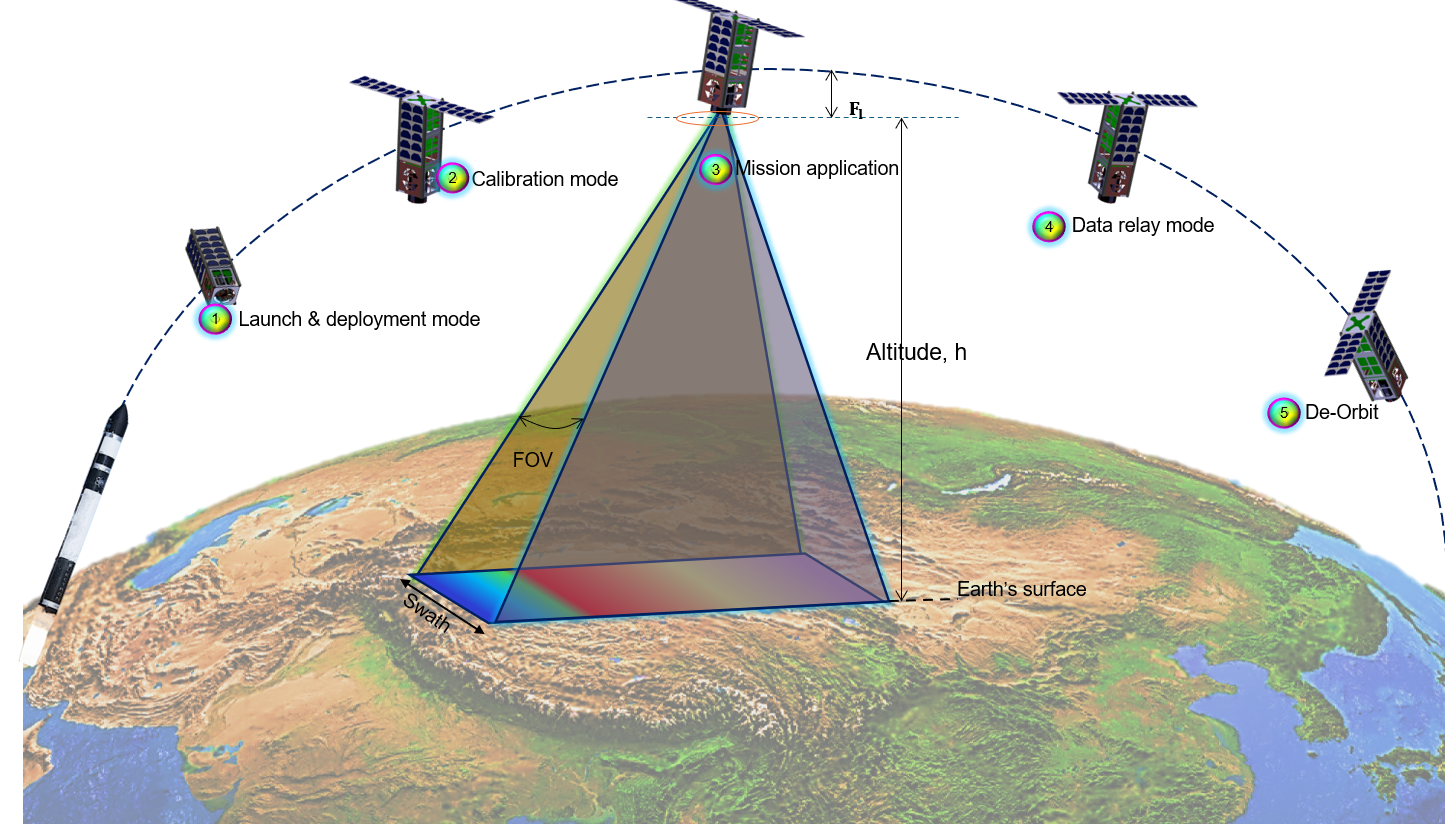
\includegraphics[width=0.48\textwidth]{figs/cubesatCOPS12.png}
	\caption{Schematic of ConOps of 3U CubeSat equipped hyperspectral optical imaging payload}
	\label{fig:ConOps}
\end{figure}
The contributions of this paper are: (i) a modified conventional Cassegrain plus on-axis prism–grating optical de sign that satisfies the 1.5U volumetric, 8–10 W power, and \(\leq 1\) kg mass constraints of a 3U CubeSat, adapting the embedded relay lens concept \cite{cheng2025nanosatellite} to a spaceborne on-axis Cassegrain fore-optic; (ii) an optomechanical integration study demonstrating a 120×100×100 mm payload envelope with modular sub-assemblies suitable for iterative qualification; and (iii) the architectural description of a proposed onboard AI data-reduction pipeline that is compatible with the SWaP headroom left available by the payload. 
\subsection{System requirements}
The target mission is a precision-agriculture Earth-observation constellation operating in a 500 km sun-synchronous orbit (SSO) with 10:30 AM local time of ascending node, providing hyperspectral coverage of cropland with revisit times short enough to support in-season crop-management decisions \cite{aragon2021cubesats, wilson2007reflecting}. The concept of operations is illustrated in Figure \ref{fig:ConOps}: after launch and deployment the payload enters an on-orbit calibration phase, then transitions to mission-application imaging over cropland targets, downlinks products through the constellation’s ground-station network, and de-orbits at end of life. %Figure \ref{fig:ConOps} demonstrates concept of operations for the hyperspectral imager from launch and deployment to Earth observation

The reflectance features relevant to precision agriculture lie predominantly in the VNIR range. Chlorophyll ab sorption at ∼450 nm (blue) and ∼670 nm (red), the green reflectance peak at ∼550 nm, the red-edge inflection at 700–740 nm and the NIR plateau at 750–850 nm collectively drive vegetation indices such as the Normalized Difference Vegetation Index (NDVI), the Normalized Difference Red-Edge index (NDRE) and the Photochemical Reflectance Index (PRI) \cite{haboudane2004hyperspectral,xue2017vegetation}. Because these features are narrow-band, hyperspectral sampling at ≤10 nm is required to resolve them cleanly; the sampling requirement in turn drives the spectrometer dispersion and slit design. The mission-level payload requirements consistent with this scenario are summarized in Table \ref{table:hsispecs}.
\section{Methodology}
\subsection{Optical design}
The optical design was developed through an iterative process that combines an inner optical loop (fore-optic, spectrometer and combined-system optimization) with an outer fabrication loop (tolerancing, optomechanical layout and fabrication), following the standard design paradigm for high-fidelity hyperspectral instruments \cite{mouroulis2018review,middleton2022holistic}. Initial first-order requirements (aperture, focal length, GSD, spectral coverage, F-number) were derived from Table \ref{table:hsispecs}, and a merit function was constructed in a commercial ray-tracing package to jointly minimize RMS spot radius and wavefront error while constraining chief-ray incidence, pupil location, vignetting and distortion \cite{smith2008modern}.
\begin{table}[h!]
	\small
	\centering
	\caption{Initial specifications of the CubeSat hyperspectral optical imaging           payload\tnote{1}}
	\label{table:hsispecs}
	\begin{threeparttable}
		\begin{tabularx}{\linewidth}{l X}
			\toprule\toprule
			\textbf{Requirement} & \textbf{Descriptions} \\ 
			\midrule
			Orbit altitude & SSO, 500 km \\
			Payload volume & \(\leq\)1.5U within a 3U CubeSat \\
			Mission & VNIR (vegetation monitoring) \\
			Spectral range & 0.488--0.85 $\mu$m \\
			Spectral sampling & 10 nm \\
			Imaging mode & Pushbroom\\
			%Across-track & \(2.2^{\circ}\) \\
			Operational F-number & F/3 target \\
			Detector format & CMOS $5.5 \mu m$, $2048 \times 2048$ pixels \\
			%Static MTF &\(\geq 0.4\) at Nyquist frequency \\
			Field of view & $\sim$2.2$^\circ$ across-track \\
			GSD at 500 km & $\sim$9.7 m at nadir \\
			Static MTF & $\geq$0.45 at 100 lp/mm \\
			Grating type & Flat prism--grating  \\
			%Envelope dimension & $\leq 100 \times 100 \times 150$ mm \\
			Imaging power consumption & $\leq$8--10 W \\
			\bottomrule\bottomrule
		\end{tabularx}
%		\begin{tablenotes}\small
%			\item[1] Initial values before design optimization.
%			\item[2] For $h=500$ km and $f_l=300$ mm, $GSD=9.7$ m requires $p\approx5.8~\mu$m.
%		\end{tablenotes}
	\end{threeparttable}
\end{table}
\subsubsection{Fore-optics design}
The fore-optics is a compact catadioptric relay based on a classical Cassegrain configuration. The Cassegrain layout was selected because its folded two-mirror geometry provides a long effective focal length within a reduced axial package, and its all-reflective front end introduces no intrinsic chromatic focal shift before the dispersive prism–grating module \cite{wilson2007reflecting,schroeder2000astronomical}. Chromatic focal shift ahead of a dispersive element would appear downstream as spectral smile, keystone, or spatial–spectral registration errors—the artefacts that most degrade hyperspectral data quality \cite{mouroulis2018review}. The primary mirror is a concave paraboloid with conic constant K1 = −1, which eliminates primary spherical aberration for an on-axis object at infinity \cite{schroeder2000astronomical}. The secondary is spherical (K2 = 0); a spherical secondary was retained to simplify fabrication, testing, and alignment, and the residual spherical aberration, coma, astigmatism and field curvature are absorbed by mirror-separation optimization and by the downstream refractive relay group, following standard third order and finite-ray aberration correction procedures \cite{smith2008modern}.

\begin{figure*}[h!]
	\centering
	\begin{minipage}[c]{1\textwidth}
		\begin{tabular}{cccc}
	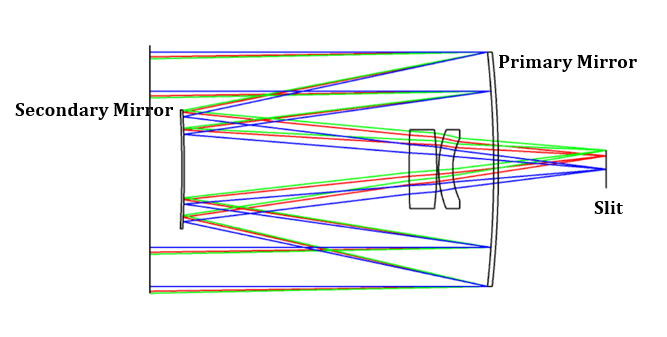
\includegraphics[width=0.48\textwidth, height=140px]{figs/Classic1.png} &
	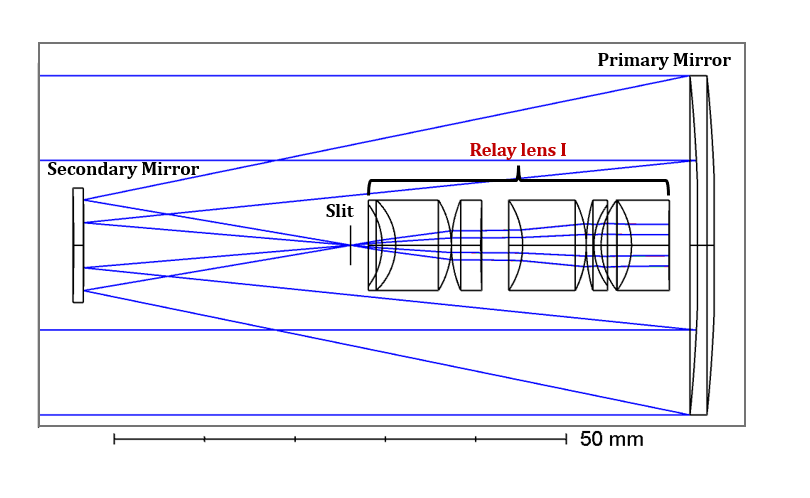
\includegraphics[width=0.48\textwidth]{figs/Modified.png} &\\
	\textbf{(a)} External image plane config. & \textbf{(b)} Internal image plane config.&\\[6pt]
		\end{tabular}
	\end{minipage}
	\caption{Cassegrain optical telescope configuration }
	\label{fig:Cassegrain}
\end{figure*}
The defining characteristic of the fore-optic, and the main architectural contribution of this study, is that the intermediate image plane is moved inside the primary-secondary envelope rather than behind the primary as in a standard Cassegrain as shown in Fig. \ref{fig:Cassegrain}. Configuration (a) corresponds to the standard external-image-plane layout utilized, for example, in the wide-spectral-range imaging spectrometer of \cite{zhang2023prismgrating}, where the intermediate image forms behind the primary through a hole in the mirror. However, in the proposed design (b), the image plane is moved forward and positioned between the primary and secondary mirrors, aligned with the spectrometer's entrance slit. This concept adapts the \text{embedded relay lens} hyperspectral architecture demonstrated at laboratory level in Ref. \cite{hsieh2011erlhis}, in which an internal relay plane replaces the conventional external scanning mechanism. %Its adaptation to a spaceborne on-axis Cassegrain fore-optic for a CubeSat payload is, to the best of our knowledge, novel.

Locating the image plane internally has three consequences that motivate the modification. First, it shortens the required separation between the telescope focus and the collimator lens group, reducing the total optical track by the axial length that would otherwise be occupied by the projection behind the primary mirror which is critical for a payload constrained to fit within a 150 mm axial envelope inside a 1.5U CubeSat allocation. Second, the internal position protects the slit plane from external mechanical protrusion and stray-light exposure. Third, the internal image plane simultaneously serves as the field stop of the complete instrument, cleanly limiting the spatial field admitted to the spectrometer without requiring a separate mechanical aperture. The trade-off is that the space between the image plane and the secondary mirror is reduced, preventing the insertion of a corrector lens close to the intermediate image; residual aberrations from the two-mirror subsystem must therefore be absorbed by the downstream collimator lens group, which is designed to serve simultaneously as a pupil relay and as an aberration corrector. Using the entrance pupil diameter \(D_{EPD}\) and working F-number N as first-order variables, the effective focal length is 
\begin{eqnarray}\label{eq:efl}
    f_{eff} = N\cdot D_{EPD}
\end{eqnarray}
For \(D_{EPD} = 75 \) mm  and \(N=3.9\) at the sensor plane, Eq. \ref{eq:efl} gives \(f_{eff} =150\) mm. The internal fore-optic operates at approximately f/1.07, delivering a fast cone to the internal slit that maximises radiometric throughput. The central obscuration ratio, 〖\(\epsilon = D_{sec}/D_{EPD}\), is minimised during layout optimisation because a larger obstruction reduces throughput and redistributes energy from the Airy core into the surrounding rings, degrading contrast at spatial frequencies below Nyquist \cite{schroeder2000astronomical}. The as-designed obscuration is ε ≈ 0.48 (linear), corresponding to an area throughput factor (\(1-\epsilon^2 \approx 0.77\)); this cost is offset in the radiometric budget by the fast internal f/1.07 throughput and by the low-groove-density transmission grating. 
\subsubsection{Spectrometer design}
The spectrometer is a transmissive prism–grating configuration, chosen over off-axis reflective alternatives for three reasons. First, transmissive elements avoid the polarisation sensitivity of oblique reflective gratings, a well-documented concern for radiometric calibration \cite{zhang2023prismgrating}. Second, the on-axis rotationally symmetric geometry preserves alignment robustness and simplifies manufacturability compared with off-axis freeform configurations \cite{xue2021underwater}. Third, the combination of a prism with a transmission grating provides a partial optical compensation of spectral smile: the inverse dispersion characteristics of the two elements can be tuned to cancel first-order smile at a design wavelength, an effect quantitatively established by Yuan et al. \cite{yuan2019airborne} for airborne prism–grating spectrometers. Energy efficiency is prioritised through a low groove density of 300 grooves/mm, which places the first diffraction order at a modest angle well-matched to the camera-group acceptance cone for the 488–850 nm range and suppresses second order overlap that would otherwise contaminate longer wavelengths \cite{yuan2019airborne}.

The fore-optic and the spectrometer are coupled at the internal image plane. Ideal ray-by-ray matching between the two subsystems is not achievable in practice; standard hyperspectral design instead enforces first-order matching of F-number and chief-ray direction at the connection plane \cite{middleton2022holistic}. Because the internal image plane is telecentric in both subsystems by construction, F-number matching alone establishes a first-order pupil match in the space of collimation. After first-order matching, all three optical groups (fore-optic, collimator, camera) were jointly re-optimised. The collimator and camera lens groups form a 4-f optical system with identical focal lengths of 20 mm, giving a slit-to-sensor length of 80 mm; combined with the fore-optic, the total optical track is 118 mm, comfortably within the 150 mm envelope. The final combined system is shown in Fig. \ref{fig:comb}.
\begin{figure}[h!]
	\centering
	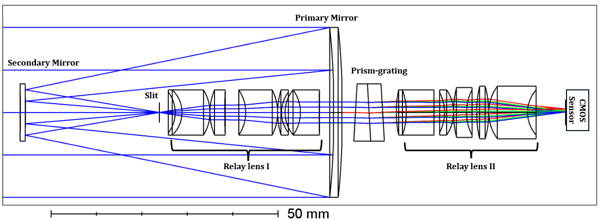
\includegraphics[width=0.45\textwidth, height=120px]{figs/Optical Label.png}
	\caption{Combined optical layout of hyperspectral imager}
	\label{fig:comb}
\end{figure}
A CMOS image sensor with 5.5 µm square global-shutter pixels, 2048×2048 format and 11.26 mm active area was selected as the focal-plane array \cite{cmv4000datasheet}. The choice is driven by the availability of windowed pushbroom-line readout, low power consumption, and prior flight heritage in comparable spaceborne instruments: this sensor family serves as the VIS-channel detector on the ASPECT hyperspectral imager for the Milani CubeSat within the ESA Hera mission \cite{nasila2025aspect}, and the same family is used in the Remote Micro-Imager of the SuperCam instrument on the Mars 2020 rover \cite{maurice2021supercam}. The pixel pitch matches the diffraction-limited spot size well: at λ = 550 nm and N =3.9, the Airy radius is 4.03 µm, so the diffraction disc is Nyquist-sampled with margin
\subsection{Optomechanical design} 
\begin{figure}[h!]
	\centering
	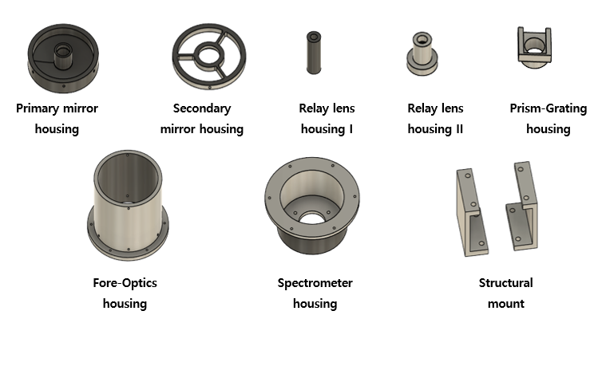
\includegraphics[width=0.45\textwidth]{figs/Parts.png}
	\caption{Optomechanical components of hyperspectral imager}
	\label{fig:opto}
\end{figure}
The optomechanical design was developed to convert the optical layout of the hyperspectral imager into a mechanically realizable and assembly-ready structure. The lens and mirror geometries designed in Zemax were exported and used as the reference optical baseline, while the mechanical housing and structural parts were modelled in Fusion 360. Each optical component, including the primary mirror, secondary mirror, relay lens groups, and prism–grating element, was first provided with an individual casing as shown in Fig. \ref{fig:opto} to ensure stable positioning, mechanical protection, and alignment compatibility.

The completed 3D model shows the full integration of the optics and barrel structure, including the fore-optics housing, spectrometer housing, structural mounts, and internal optical supports. This design process ensured that the hyperspectral imager was not only optically valid but also mechanically manufacturable, alignable, and suitable for further structural and tolerance analysis.
\begin{figure}[h!]
	\centering
	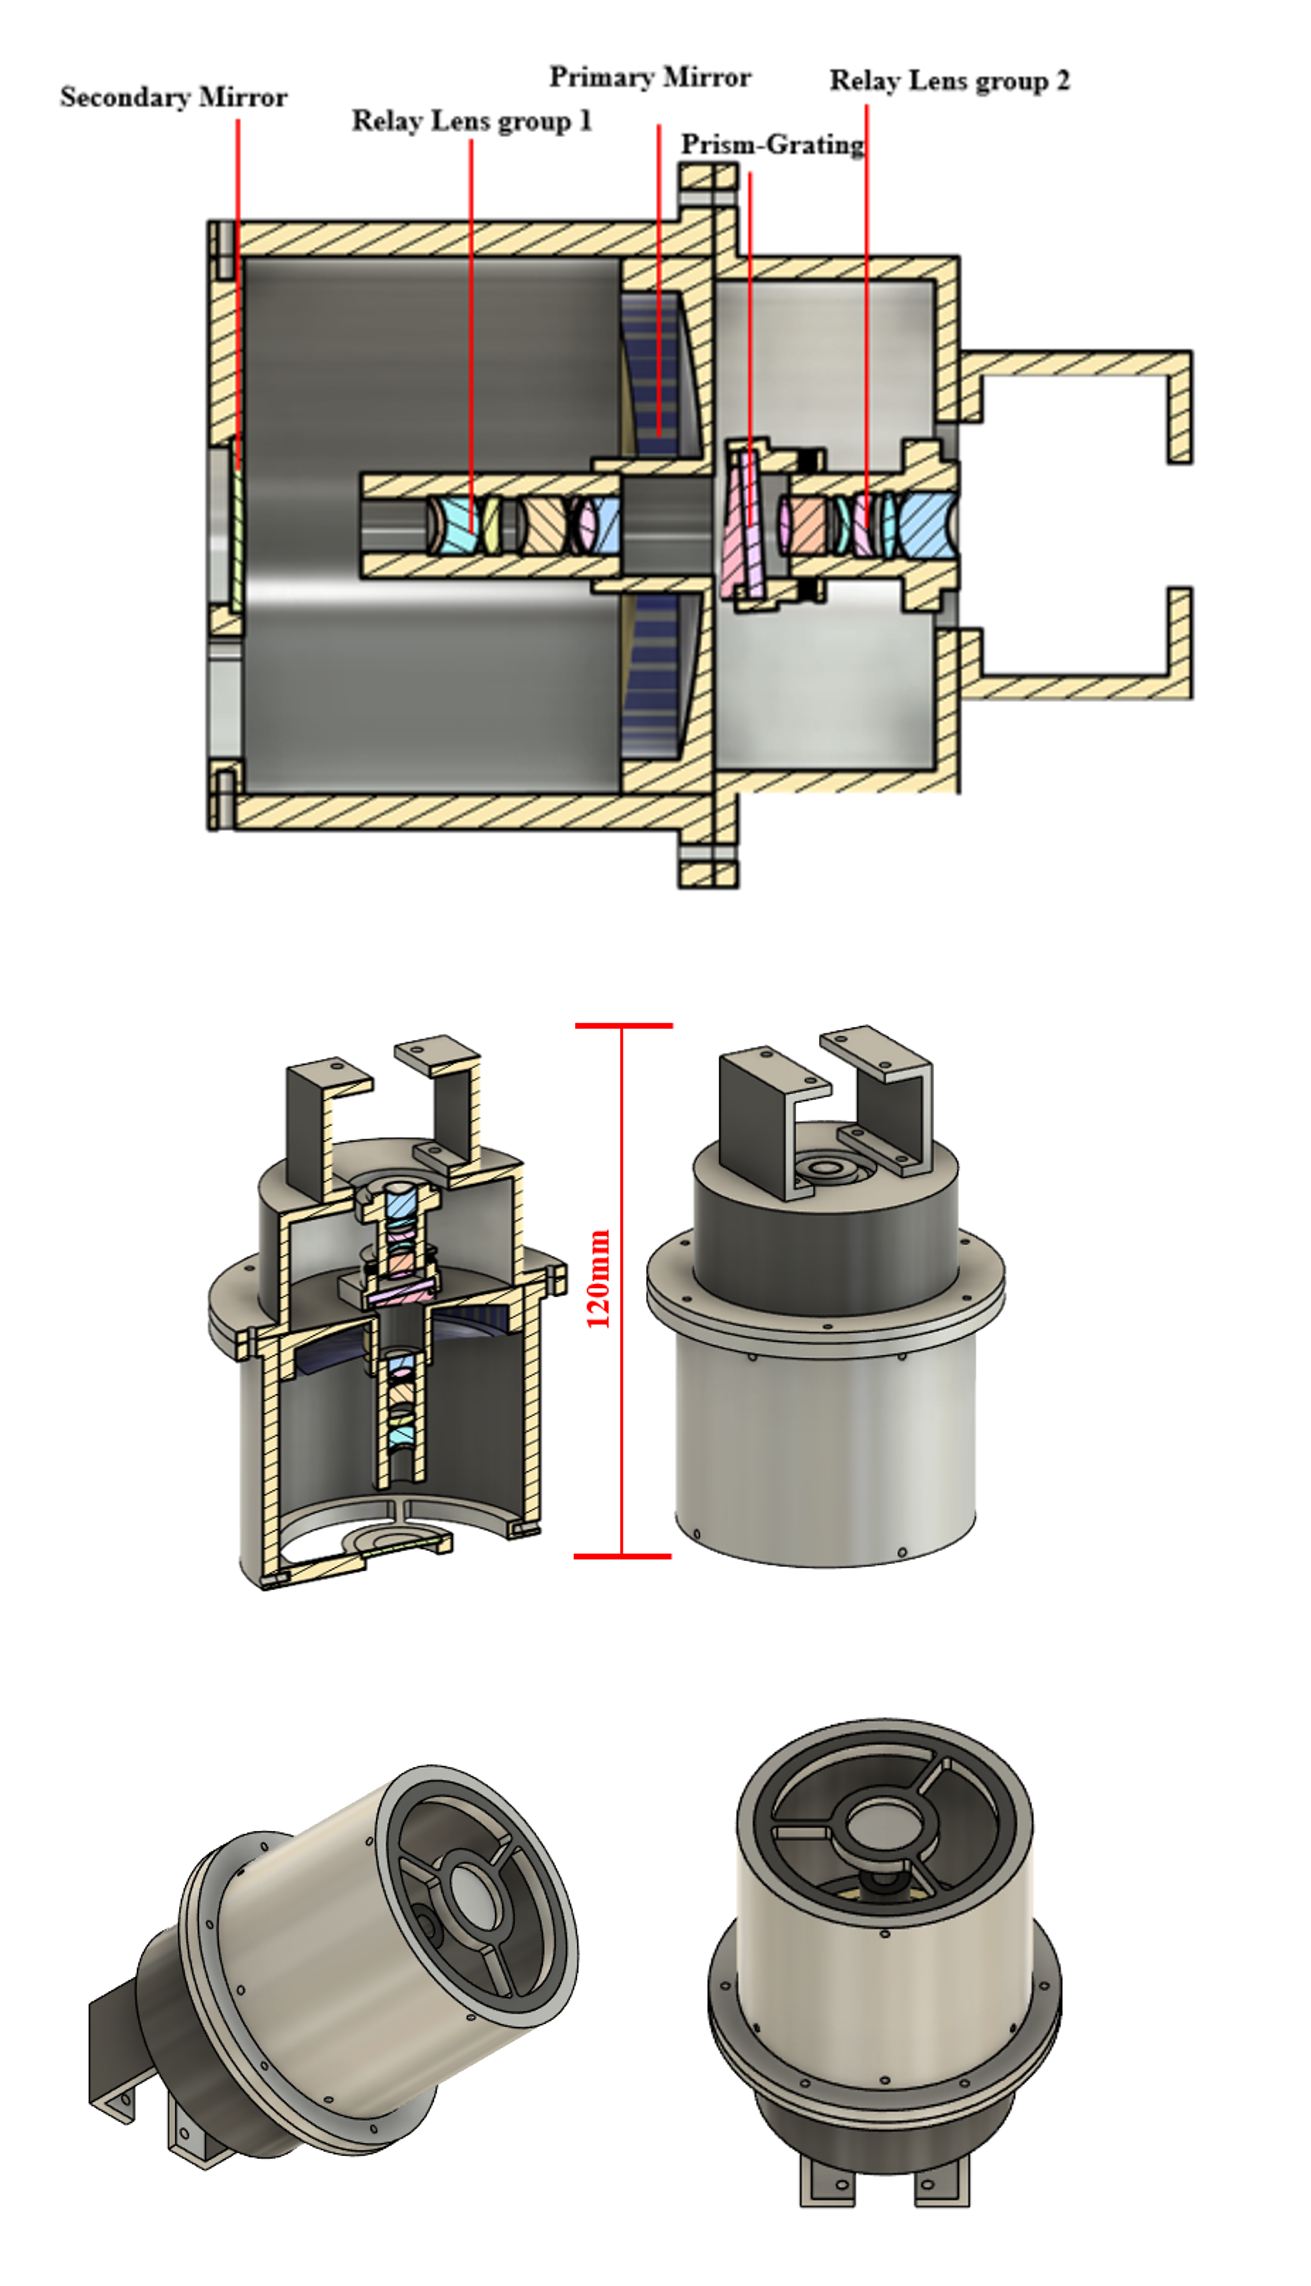
\includegraphics[width=0.45\textwidth]{figs/Optomechanical.png}
	\caption{Optomechanical assembled and sectional view of Hyperspectral imager}
	\label{fig:optoa}
\end{figure}
For the mechanical casing, Aluminium 6061 was selected. The upper casing, which supports the mirror section, was designed using black anodized AL6061. The black anodized surface reduces internal reflection and stray light within the optical path. The lower casing, which houses the grating and sensor section, was fabricated using non-painted aluminium. This allowed the structure to maintain sufficient mechanical strength while supporting the optical components and detector assembly. Table 2 lists the opto-mechanical properties of the materials. Through this selection process, the material configuration was optimized to balance optical performance, structural integrity, thermal stability, and fabrication feasibility.

\subsection{Onboard AI-based conceptual architecture}
Consider an Earth-observation mission in which each acquisition produces a raw hyperspectral product \(P_0\)
\begin{figure*}[h!]
	\centering\includegraphics[width=0.9\textwidth]{figs/fig1}
	\caption{Conceptual proposed on-board AI processing architecture}% (adapted with permission from Ref. \cite{Cao2020}) (\textcolor{red}{produce your own perspective)}}
\label{fig:concept}
\end{figure*}
An onboard processor may convert \(P_0\) into one of three lower-volume mission products: an ROI-cropped cube \(P_1\), a segmentation raster \(P_2\), or a semantic alert \(P_3\) containing only decision-relevant metadata, such as class, location, area, confidence, and acquisition time. For an onboard model \(m \in \mathcal{M}\) and product tier \(p \in \mathcal{P} = \{0,1,2,3\}\), the selected mission product is expressed as
\begin{eqnarray}
P_p = g_{m,p}(P_0)
\end{eqnarray}
where \(g_{m,0}\) is the identity mapping for conventional raw-cube downlink and \(g_{m,p}\),  \(p \in \mathcal{P} = \{0,1,2,3\}\) denotes the onboard transformation used to generate the corresponding reduced product.

The mission-design objective is to reduce the amount of data transmitted to the ground and the time required to deliver actionable information, while maintaining sufficient task performance and remaining within onboard resource limits. Because data volume, latency, energy, and semantic risk have different physical units, the trade is expressed using a normalized mission-level cost function:
\begin{eqnarray}\label{eq:costfunc}
\begin{aligned}
	\mathcal{J}(m,p) = w_D \frac{D_p}{D_0} + w_L \frac{L_{post}(m,p)}{L_{req}} \\+ w_E \frac{E_{proc}(m,p)}{E_{avail}} + w_R \mathcal{\hat{R}}_{sem}(m,p)
\end{aligned}
\end{eqnarray}
Here \(D_p\) is the size of the selected product, \(D_0\) is the raw-cube size, \(L_{post}(m,p)\) is the post-acquisition latency required to deliver the selected product, \(L_{req}\) is the maximum acceptable mission latency, \(E_{proc}(m,p)\) is the onboard processing energy required to generate the product, and \(E_{avail}\) is the energy allocated to processing one observation. The normalized semantic-risk term \(\mathcal{\hat{R}}_{sem}(m,p) \in [0,1]\) represents the operational risk associated with replacing the original measurement with a task-specific product, including missed events, false alarms, geolocation errors, model drift, and loss of information required for subsequent scientific analysis.

Figure \ref{fig:concept} shows the source concept: a constellation acquires hyperspectral data, runs an onboard segmentation engine, converts the segmentation to ROI information, and transmits a compact text payload. The mission architecture refined here adds three operational rules. First, \(P_0\) is retained locally until a retention deadline or positive ground acknowledgement. Second, \(P_3\) is placed in a high-priority queue only when confidence and quality gates are satisfied; otherwise, the system marks the event uncertain and schedules \(P_1\) or \(P_0\). Third, the ground segment can request evidence products after receiving the alert.

The end-to-end workflow is: (1) acquire and calibrate the cube; (2) associate time and geometry; (3) execute segmentation; (4) extract connected ROIs and attributes; (5) apply confidence, quality, and safety gates; (6) generate P3 and store references to P0/P1; (7) insert products into a contact-aware priority queue; (8) transmit P3 at the next feasible contact; and (9) trigger ground alerting, follow-up tasking, or evidence retrieval. This two-tier workflow limits the consequence of an erroneous model output because the underlying measurement remains available.
A practical packet should also include an integrity check, schema version, model hash, processing timestamp, spacecraft and sensor identifiers, and explicit units. Geographic coordinates should not be generated from segmentation alone; they require a validated geolocation chain and associated uncertainty. These fields are minor in volume but central to operational trust, cross-satellite fusion, and post-event audit.
\section{Results and discussion}
\subsection{Modulation transfer function}
The system-level imaging performance of the payload is evaluated in terms the Modulation Transfer Function (MTF), signal-to-noise ratio (SNR). The system MTF at the detector plane was modelled as a product of the principal image-chain contributions, including diffraction, residual aberration, detector sampling, motion smear, and line-of-sight jitter. Under the assumption that these effects can be treated as independent linear shift-invariant degradations along the evaluated spatial-frequency direction, the system MTF is approximated as
\begin{eqnarray}
	\begin{split}
		MTF_{sys} =  & \alpha \cdot MTF_{opt} \cdot MTF_{det} \cdot MTF_{mot} \\
		&  \cdot MTF_{jit} \cdot MTF_{elec}
	\end{split}
	\label{eqn:mtf_system}
\end{eqnarray}
where \(\mathrm{\alpha}\) represents manufacturing and alignment loss, \(MTF_{opt}\) is the optical MTF, \(MTF_{det}\) is the detector MTF, \(MTF_{jit}\) represents pointing jitter,  and \(MTF_{mot}\) represents image smear due to platform motion, and \( MTF_{elec}\) represents electronic filtering. For a diffraction-limited circular aperture, the image-plane optical diffraction MTF at image plane is:
\begin{eqnarray} 
	\begin{aligned}
	M_{diff} =
	\begin{cases}
		\displaystyle \frac{2}{\pi} \left[\cos^{-1}\left(\frac{\upsilon}{\upsilon_c}\right) - \frac{\upsilon}{\upsilon_c}
		\sqrt{1-\left(\frac{\upsilon}{\upsilon_c}\right)^2}\right] \\%[11pt]
		0\leq \upsilon \leq \upsilon_c, \qquad \frac{\upsilon}{\lambda N}	
	\end{cases}
	\end{aligned}
	\label{eqn:diff_mtf}
\end{eqnarray}
where \(\upsilon\) is the image-plane spatial frequency. For incoherent imaging, the diffraction cutoff frequency is \(\upsilon_c  = \frac{1}{\lambda F/\#}.\) This form is appropriate for estimating MTF in cycles/mm or lp/mm at the detector plane. Assuming a square detector aperture with effective width equal to the pixel pitch p, the detector MTF is approximated as:
\begin{eqnarray}
	M_{det} =  \frac{\sin({\pi \times FoV \times f})}{\pi \times FoV\times f} \triangleq \left|
	\frac{\sin(\pi f p)}{\pi f p}
	\right|
	\label{eqn:detector_mtf}
\end{eqnarray}
where the detector Nyquist frequency is represented as \(f_N = \frac{1}{2p}.\). For the selected detector pitch of \(p=5.5 \mu m\), the detector Nyquist frequency is
\begin{eqnarray}
	\upsilon_{Nsq} = \frac{1}{2p} = \frac{90lp}{mm}
\end{eqnarray} 
The as-designed on-axis MTF at Nyquist across the 488–850 nm range is shown in Fig. \ref{fig:mtf}, together with the requirement threshold of Table \ref{table:hsispecs}. The system exceeds MTF = 0.4 at Nyquist at all three representative wavelengths. 
\begin{figure}[h!]
	\centering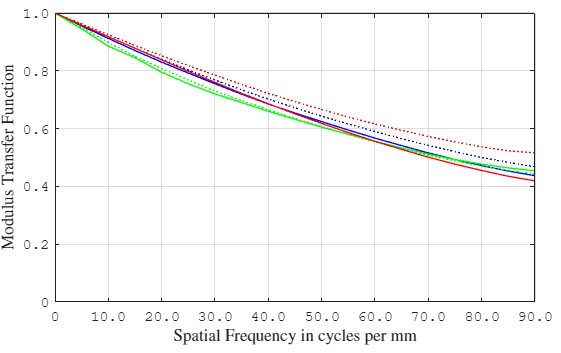
\includegraphics[width=0.45\textwidth]{figs/MTF}
	\caption{Modulation transfer function of optical imager}
	\label{fig:mtf}
\end{figure}
\subsection{Signal-to-noise ratio}
The signal collected by a single detector pixel per pushbroom line, in units of photoelectrons, for a spectral band centred at \(\lambda\) with bandpass \(\Delta \lambda\), is 
\begin{eqnarray}
	\begin{aligned}
	S(\lambda) = L_{TOA}(\lambda) \cdot \frac{\pi}{4N^2}\cdot (1-\epsilon^2)\cdot \tau\cdot \Delta\lambda \\
	\cdot \eta_{opt}(\lambda) \cdot\eta_q(\lambda)\cdot\frac{\lambda}{hc}
	\end{aligned}
\end{eqnarray}
where \( L_{TOA}(\lambda)\) is the top-of-atmosphere spectral radiance \(Wm^{-2}sr^{-1}nm^{-1}\), \(N\) is the working F-number, ε is the linear central obscuration, \(A_{px}=p^2\) is the pixel area, \(\tau\) is the integration time, \(\eta_{opt}(\lambda)\) is the end-to end optical throughput (mirror reflectance, prism transmission, grating efficiency, slit losses and coatings), \(\eta_q(\lambda)\) is the detector quantum efficiency, and \(\frac{\lambda}{hc}\) is the photon energy \cite{mouroulis2018review,ieee2012icsai}. For a Lambertian ground scene of reflectance \(\rho\) under solar zenith angle \(\theta_s\) and one-way atmospheric transmission \(T_{atm} (\lambda)\), the top-of-atmosphere radiance is
\begin{eqnarray}
	 L_{TOA}(\lambda) (\lambda) = \frac{E_{\odot}(\lambda)\cos\theta_s\cdot\rho\cdot T_{atm}(\lambda)}{\pi}
\end{eqnarray}
where \(E_{\odot}(\lambda)\) is the exo-atmospheric solar spectral irradiance. The total noise in electrons per pixel per line combines shot noise, dark-current noise and read noise as well as the resulting per-pixel per-band signal-to-noise ratio is 
\begin{eqnarray}
	\begin{aligned}
	\sigma(\lambda) = \sqrt{S(\lambda) + N_{dt} +N_r^2}\\
	SNR(\lambda) = \frac{S(\lambda)}{\sigma(\lambda)}
	\end{aligned}
\end{eqnarray}
Under representative sun-synchronous illumination conditions (\(\theta_s = 30^{\circ}, \rho=0.3\)) reference reflectance, mid latitude summer atmosphere) and using the sensor and optical parameters of Table \ref{table:hsispecs}, the computed SNR as a function of wavelength is shown in Fig. \ref{fig:snr}. 
\begin{figure}[h!]
	\centering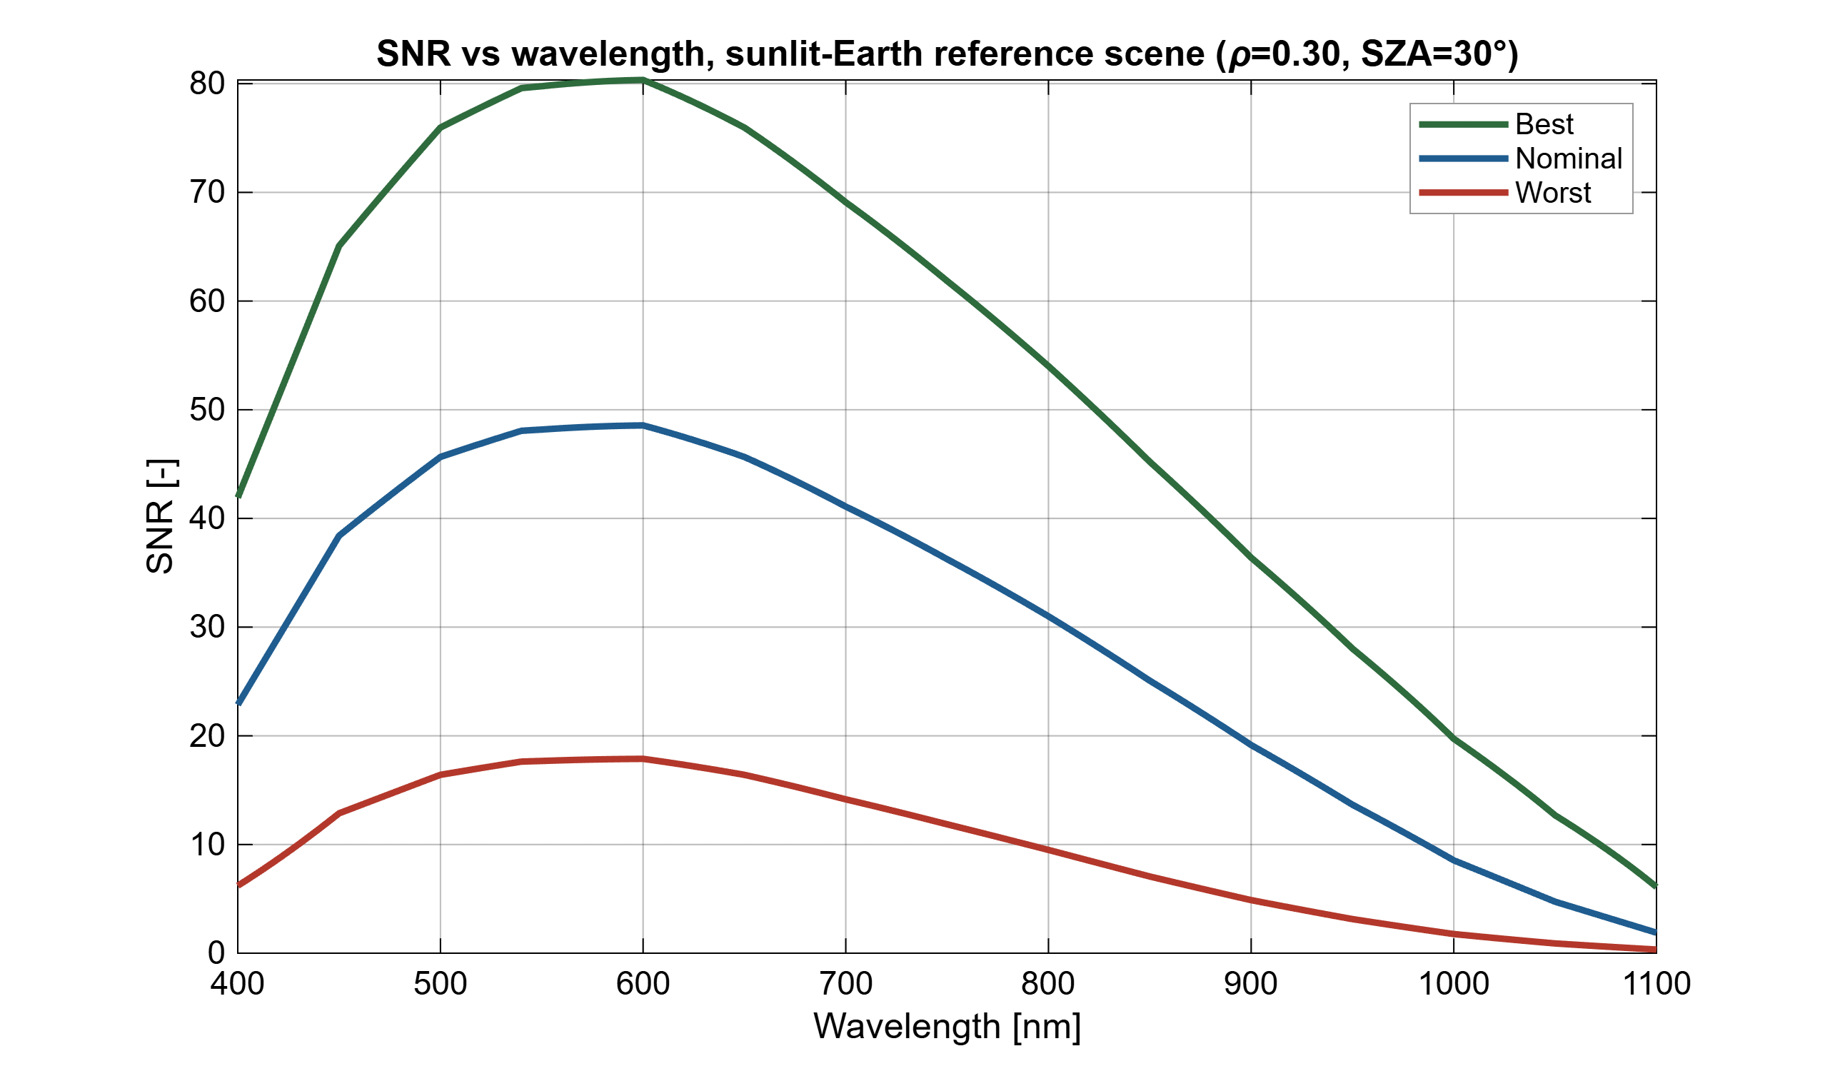
\includegraphics[width=0.45\textwidth]{figs/SNR.png}
	\caption{Signal-to-ratio of optical imager across wavelengths}
	\label{fig:snr}
\end{figure}
The SNR peaks near 600 nm and falls toward both edges of the band. The peak location is set by the product of the solar irradiance, the optical transmission, and the quantum efficiency, all of which are strongest in the green to red. The fall toward the blue is driven by the declining quantum efficiency below 450 nm, while the long roll-off into the near-infrared follows the steep collapse of the silicon response beyond about 900 nm. In the nominal case the peak SNR is about 49, the band average is about 30, and the value holds above 25 across from 450 to 900 nm core where most spectral information of interest sits.
\begin{figure*}[h!]
	\centering
	\begin{minipage}[c]{1\textwidth}
		\begin{tabular}{cccc}
			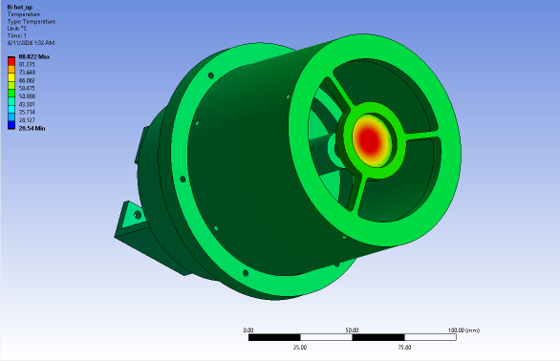
\includegraphics[width=0.28\textwidth, height=110px]{figs/Hot operational case temperature field.png} &
			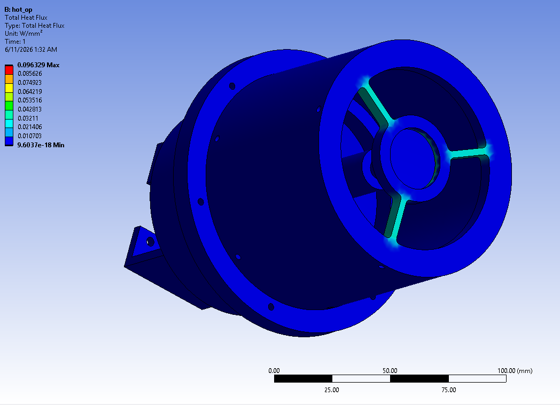
\includegraphics[width=0.28\textwidth, height=110px]{figs/. Hot operational case total heat flux.png} &
			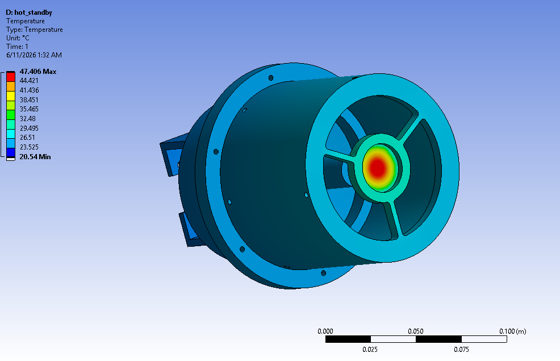
\includegraphics[width=0.28\textwidth, height=110px]{figs/Hot standby case temperature field.png} &\\
			\textbf{(a)} Hot operational case temperature field & \textbf{(b)} Hot operational case total heat flux &  \textbf{(c)} Hot standby case temperature field &\\[6pt]
			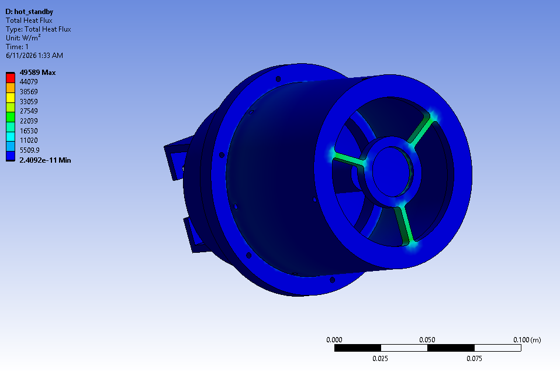
\includegraphics[width=0.28\textwidth, height=110px]{figs/Hot standby case total heat flux.png} &
			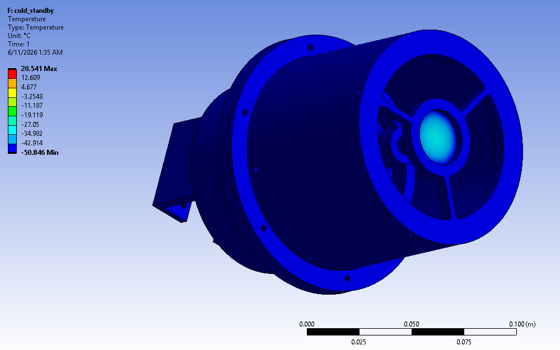
\includegraphics[width=0.28\textwidth, height=110px]{figs/Cold standby case temperature field.png} &
			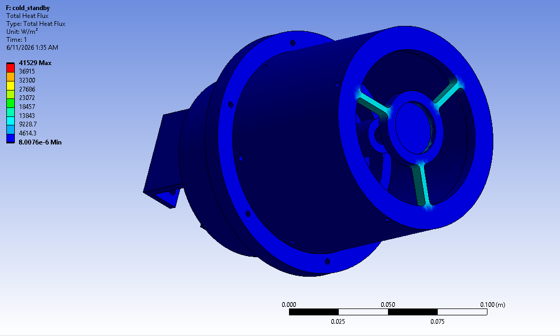
\includegraphics[width=0.28\textwidth, height=110px]{figs/Cold standby case total heat flux..png} &\\
			\textbf{(d)} Hot standby case total heat flux & \textbf{(e)} Cold standby case temperature field &  \textbf{(f)} Cold standby case total heat flux &\\[6pt]
		\end{tabular}
	\end{minipage}
	\caption{Steady-sate thermal analysis results}
	\label{fig:thermal}
\end{figure*}
\subsection{Thermal analysis}
The temperature extremes for the three cases are shown in Fig.~\ref{fig:thermal}. The pattern is exactly what physics predicts. The sunlit anodized section is the hottest region in both hot cases, the deep space facing and bus facing surfaces are the coldest, the cold case sits below the hot cases throughout, and the metal is nearly isothermal in every case. The maximum gradient across the metal is well below the 1.5 degrees Celsius uniformity reference of the methodology, which the low Biot number guarantees.
\subsection{Fabrication and prototype}
The designed components were sent to industrial fabrication partners for manufacturing. The fabrication process focused on producing the optical and mechanical parts according to the finalized fabrication data while preserving the required alignment accuracy of the hyperspectral imager.
The fabricated prototype as shown in Fig.~\ref{fig:expsetup} consisted of the main case barrel, primary mirror holder, secondary mirror holder, camera mount, and assembled optical body. The main case barrel formed the primary structural housing of the telescope section. The primary and secondary mirror holders were fabricated separately to allow precise positioning of the reflective elements inside the Cassegrain configuration. The camera mount was also fabricated as an independent component to support the detector alignment with respect to the final image plane

The fabrication stage therefore validated the transition from optical design to physical implementation. By using the selected materials and fabrication-ready optical prescription, the prototype was manufactured in a form suitable for further alignment, laboratory testing, and performance verification. This process demonstrated the practical feasibility of implementing a CubeSat-compatible hyperspectral imager using the proposed optical and mechanical design.

The fabricated prototype consisted of the main case barrel, primary mirror holder, secondary mirror holder, camera mount, and assembled optical body. The main case barrel formed the primary structural housing of the telescope section. The primary and secondary mirror holders were fabricated separately to allow precise positioning of the reflective elements inside the Cassegrain configuration. The camera mount was also fabricated as an independent component to support the detector alignment with respect to the final image plane.
%\begin{figure}[h!]
%	\centering
%	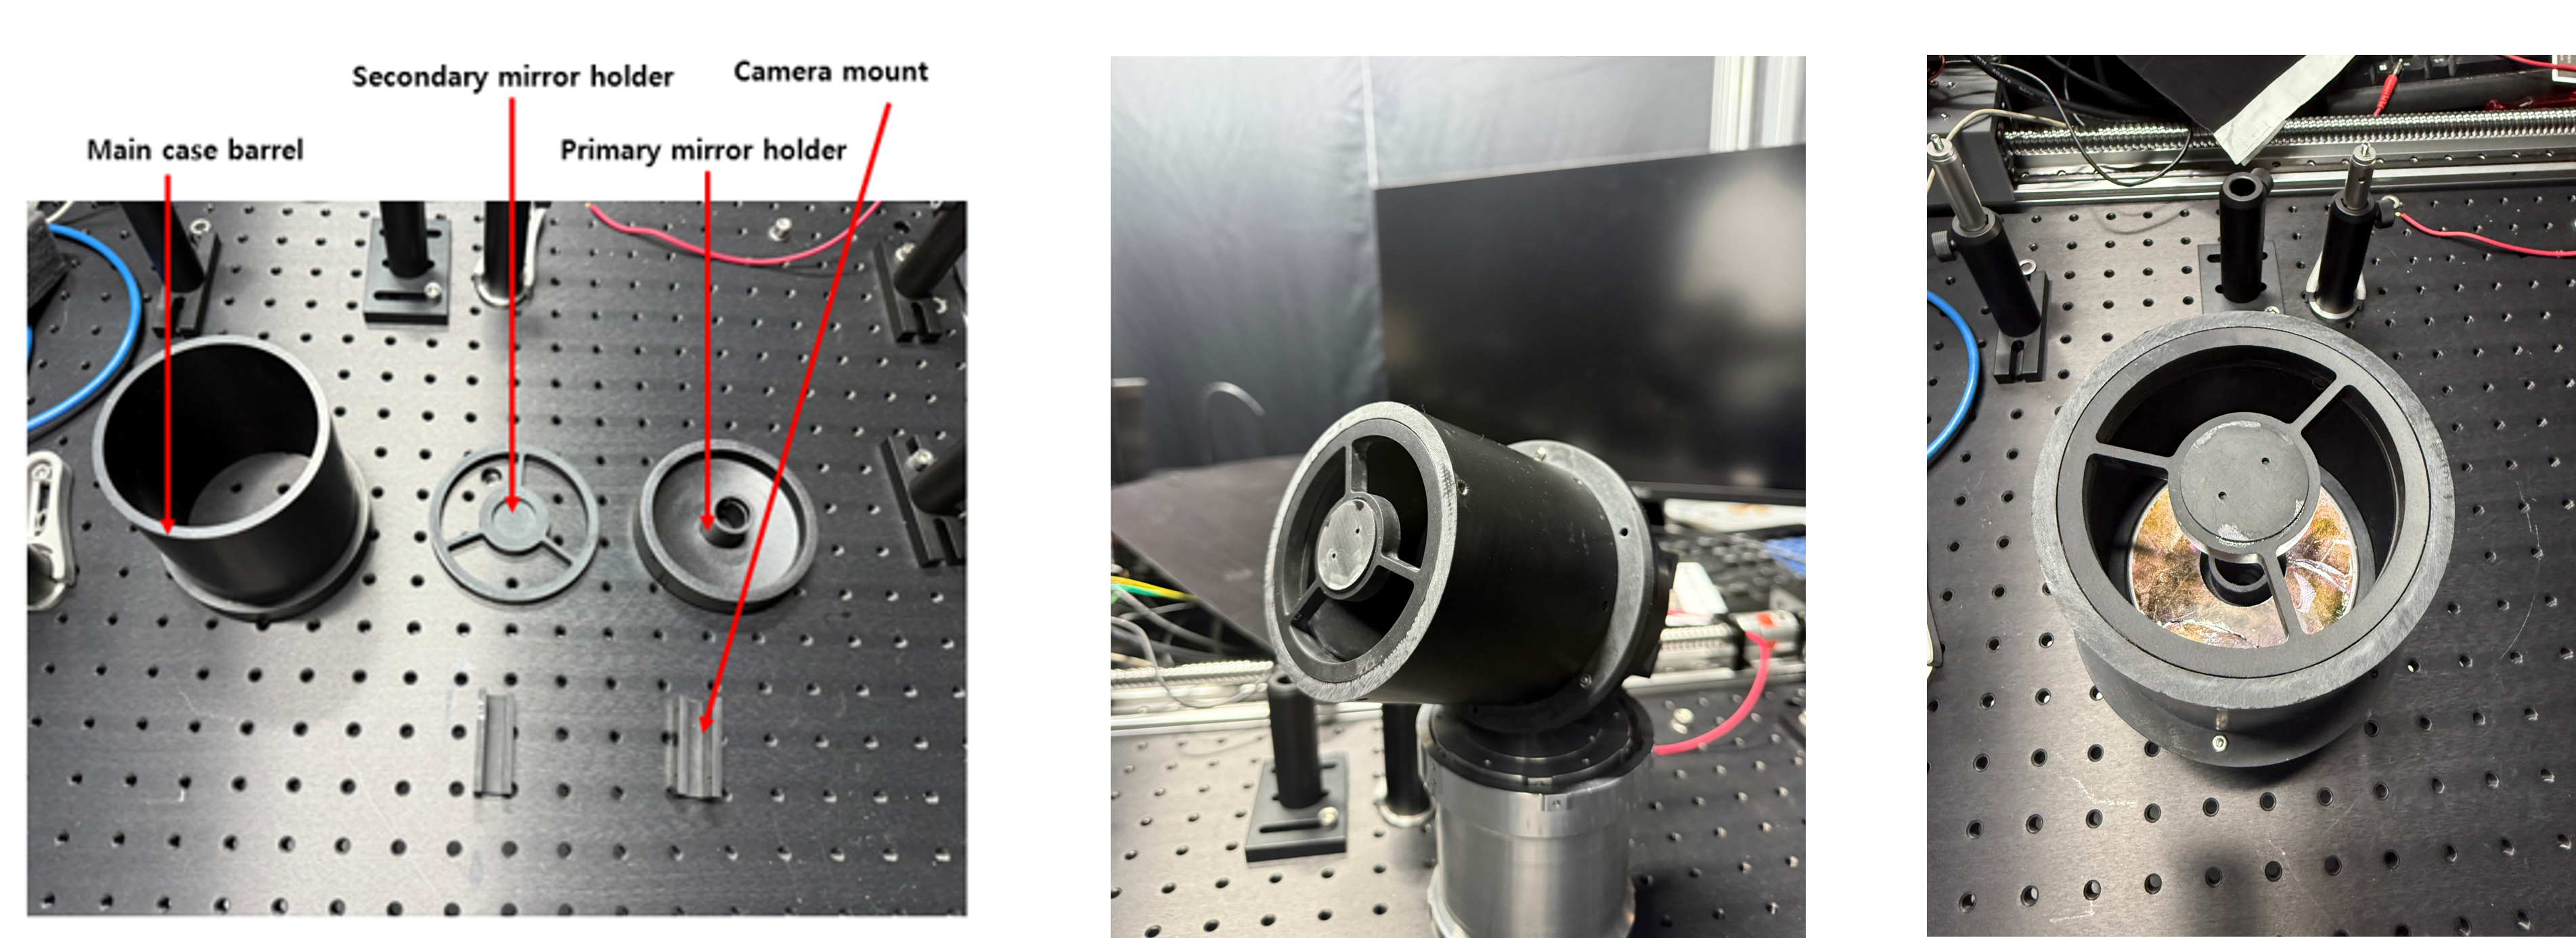
\includegraphics[width=0.45\textwidth]{figs/Expt.png}
%	\caption{Optomechanical assembled and sectional view of Hyperspectral imager}
%	\label{fig:optoa}
%\end{figure}
\begin{figure*}[t]
	\centering
	% Three equal-width boxes spread evenly across the full text width:
	% 3 x 0.31 = 0.93\textwidth of content, the remaining 0.07 split into two
	% identical \hfill gaps.  Giving \includegraphics only a height keeps every
	% photograph at its natural aspect ratio, and the shared height makes the
	% row line up.  The rotated photographs are scaled BEFORE they are rotated
	% (width= listed before angle=), so their 40mm width becomes the final
	% height and the row stays even.  angle= before height= overflows
	% graphicx on images this large ("Division by 0").
	\begin{subfigure}[b]{0.33\textwidth}
		\centering
		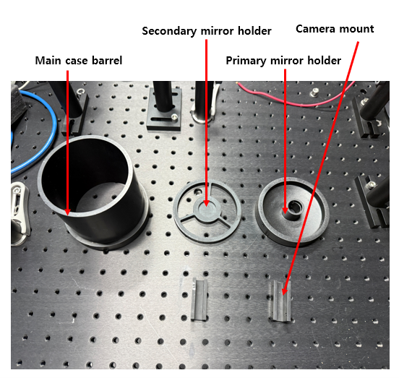
\includegraphics[width=45mm]{figs/Label1.png}
		\caption{Fabricated components }
	\end{subfigure}
	\hfill
	\begin{subfigure}[b]{0.33\textwidth}
		\centering
		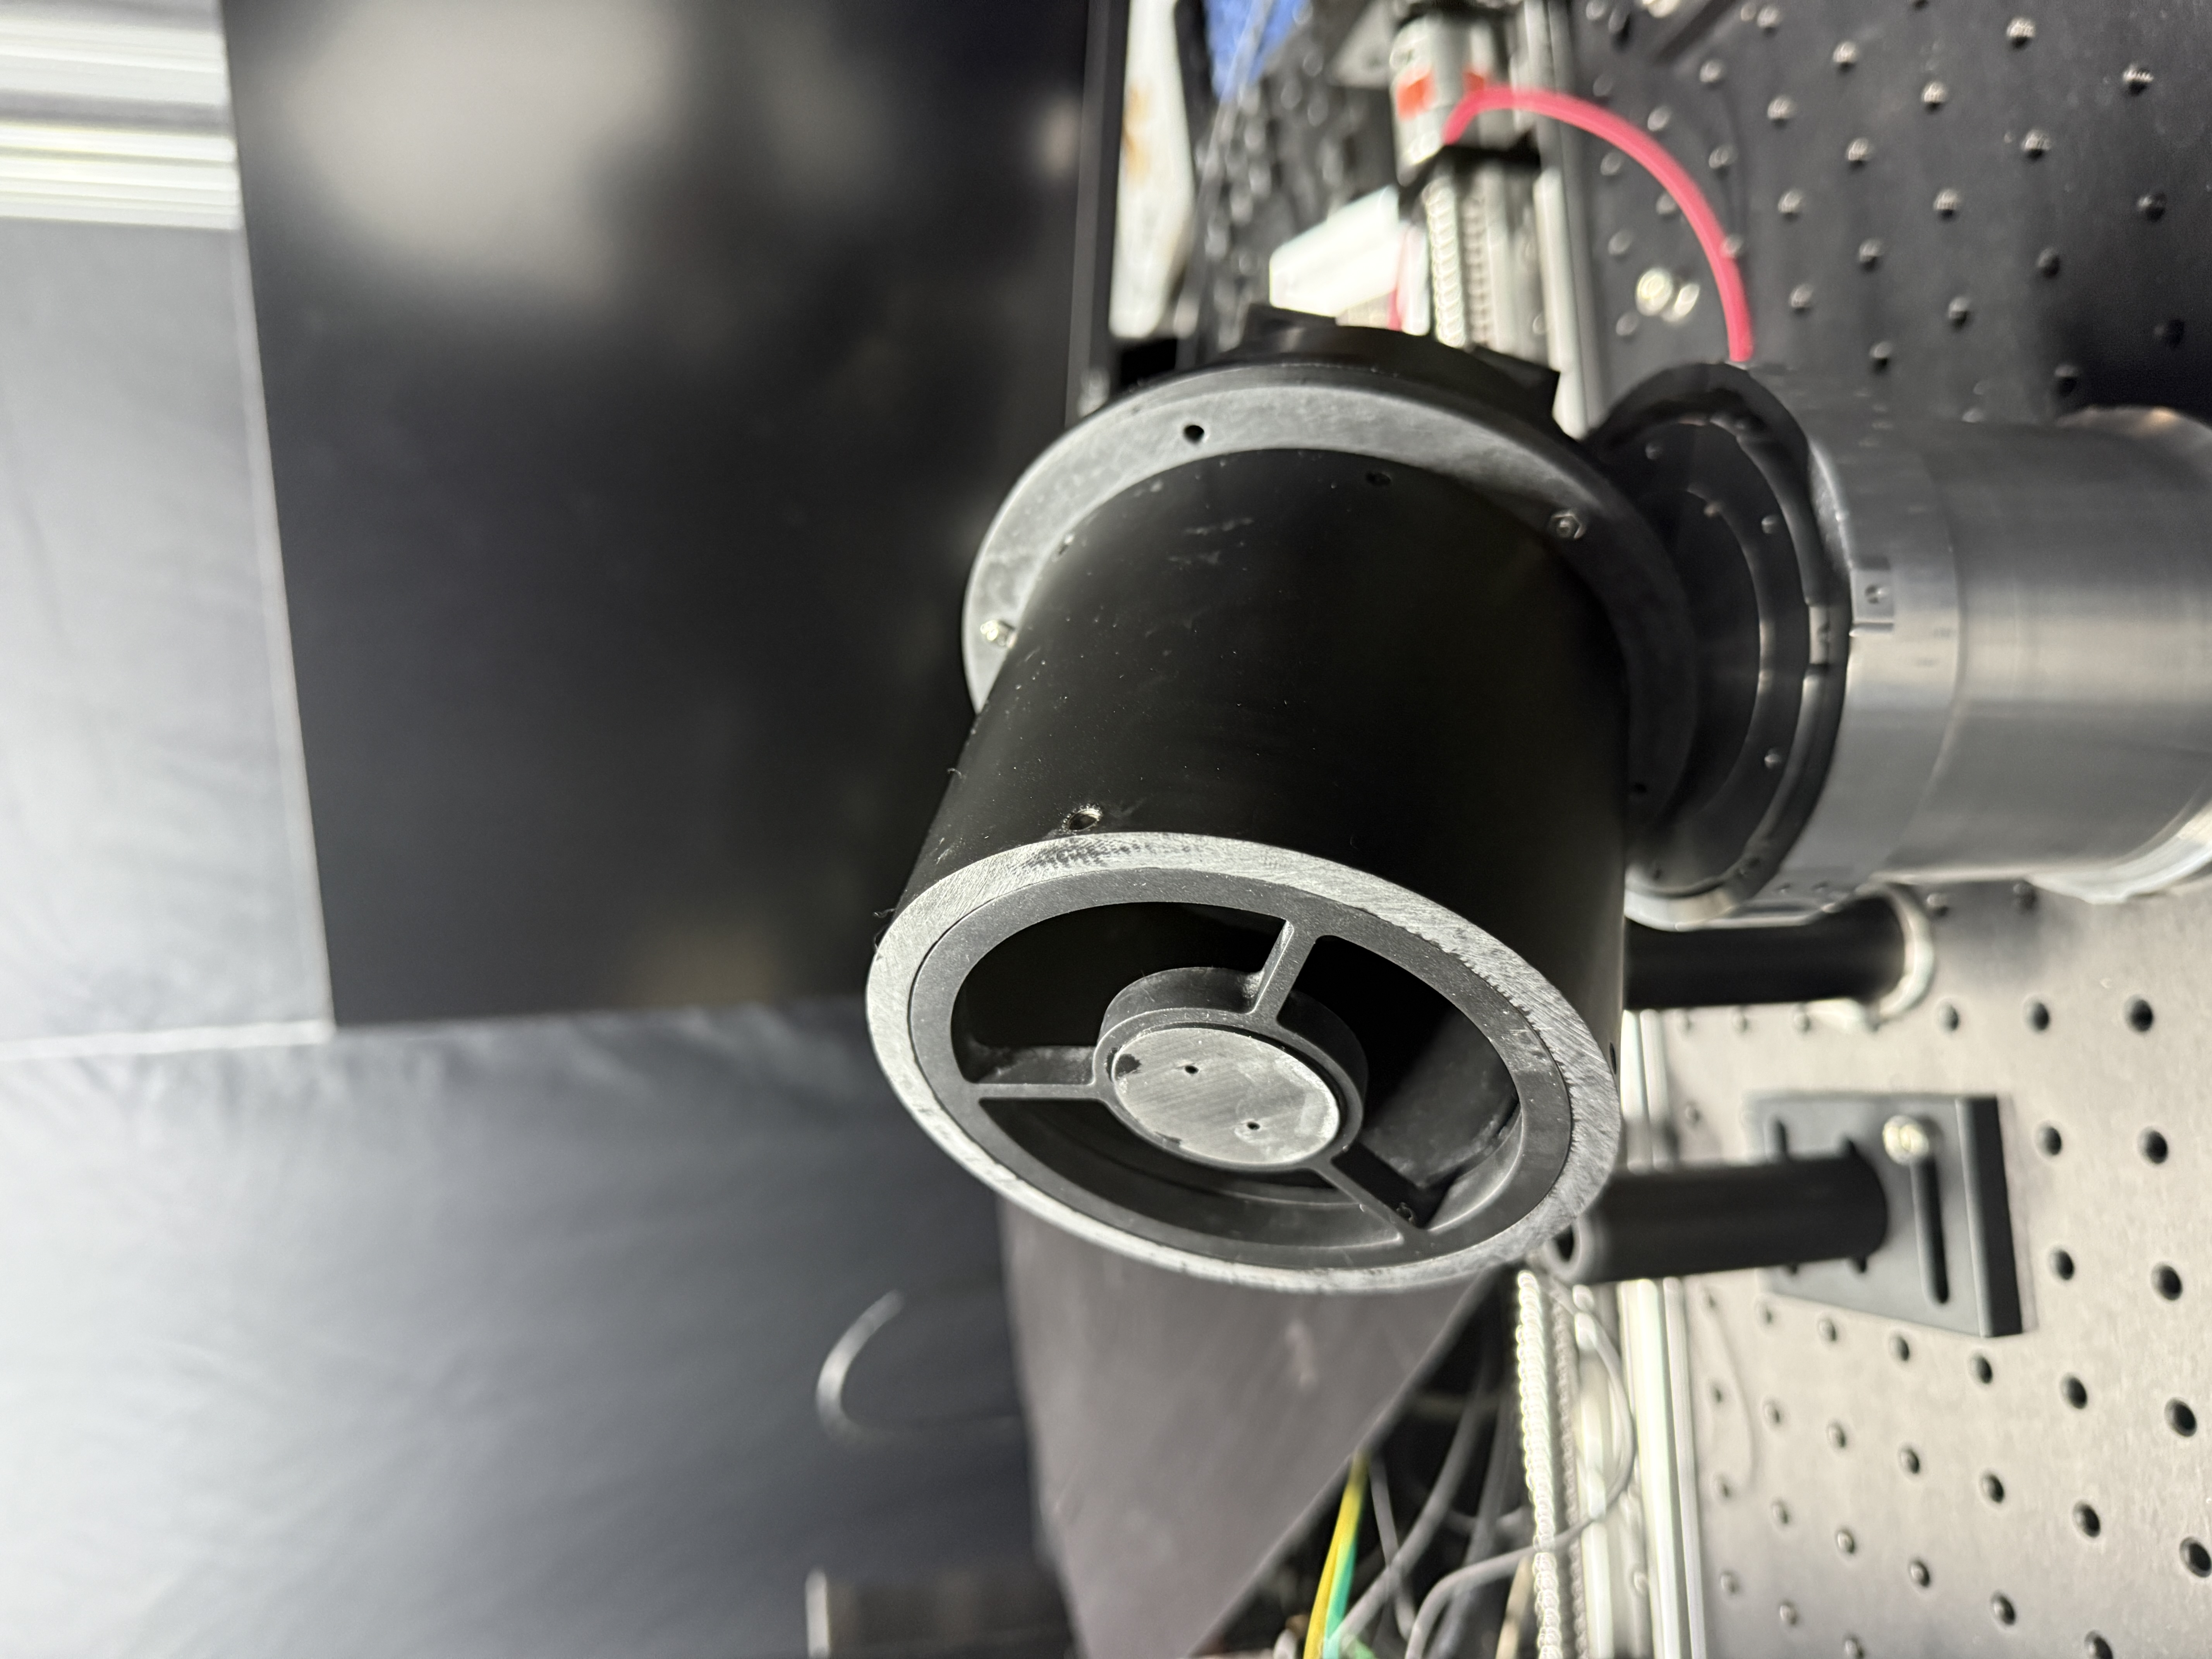
\includegraphics[width=45mm,angle=-90]{figs/Exp4.jpg}
		\caption{Fabricated assembly }
	\end{subfigure}
	\hfill
	\begin{subfigure}[b]{0.33\textwidth}
		\centering
		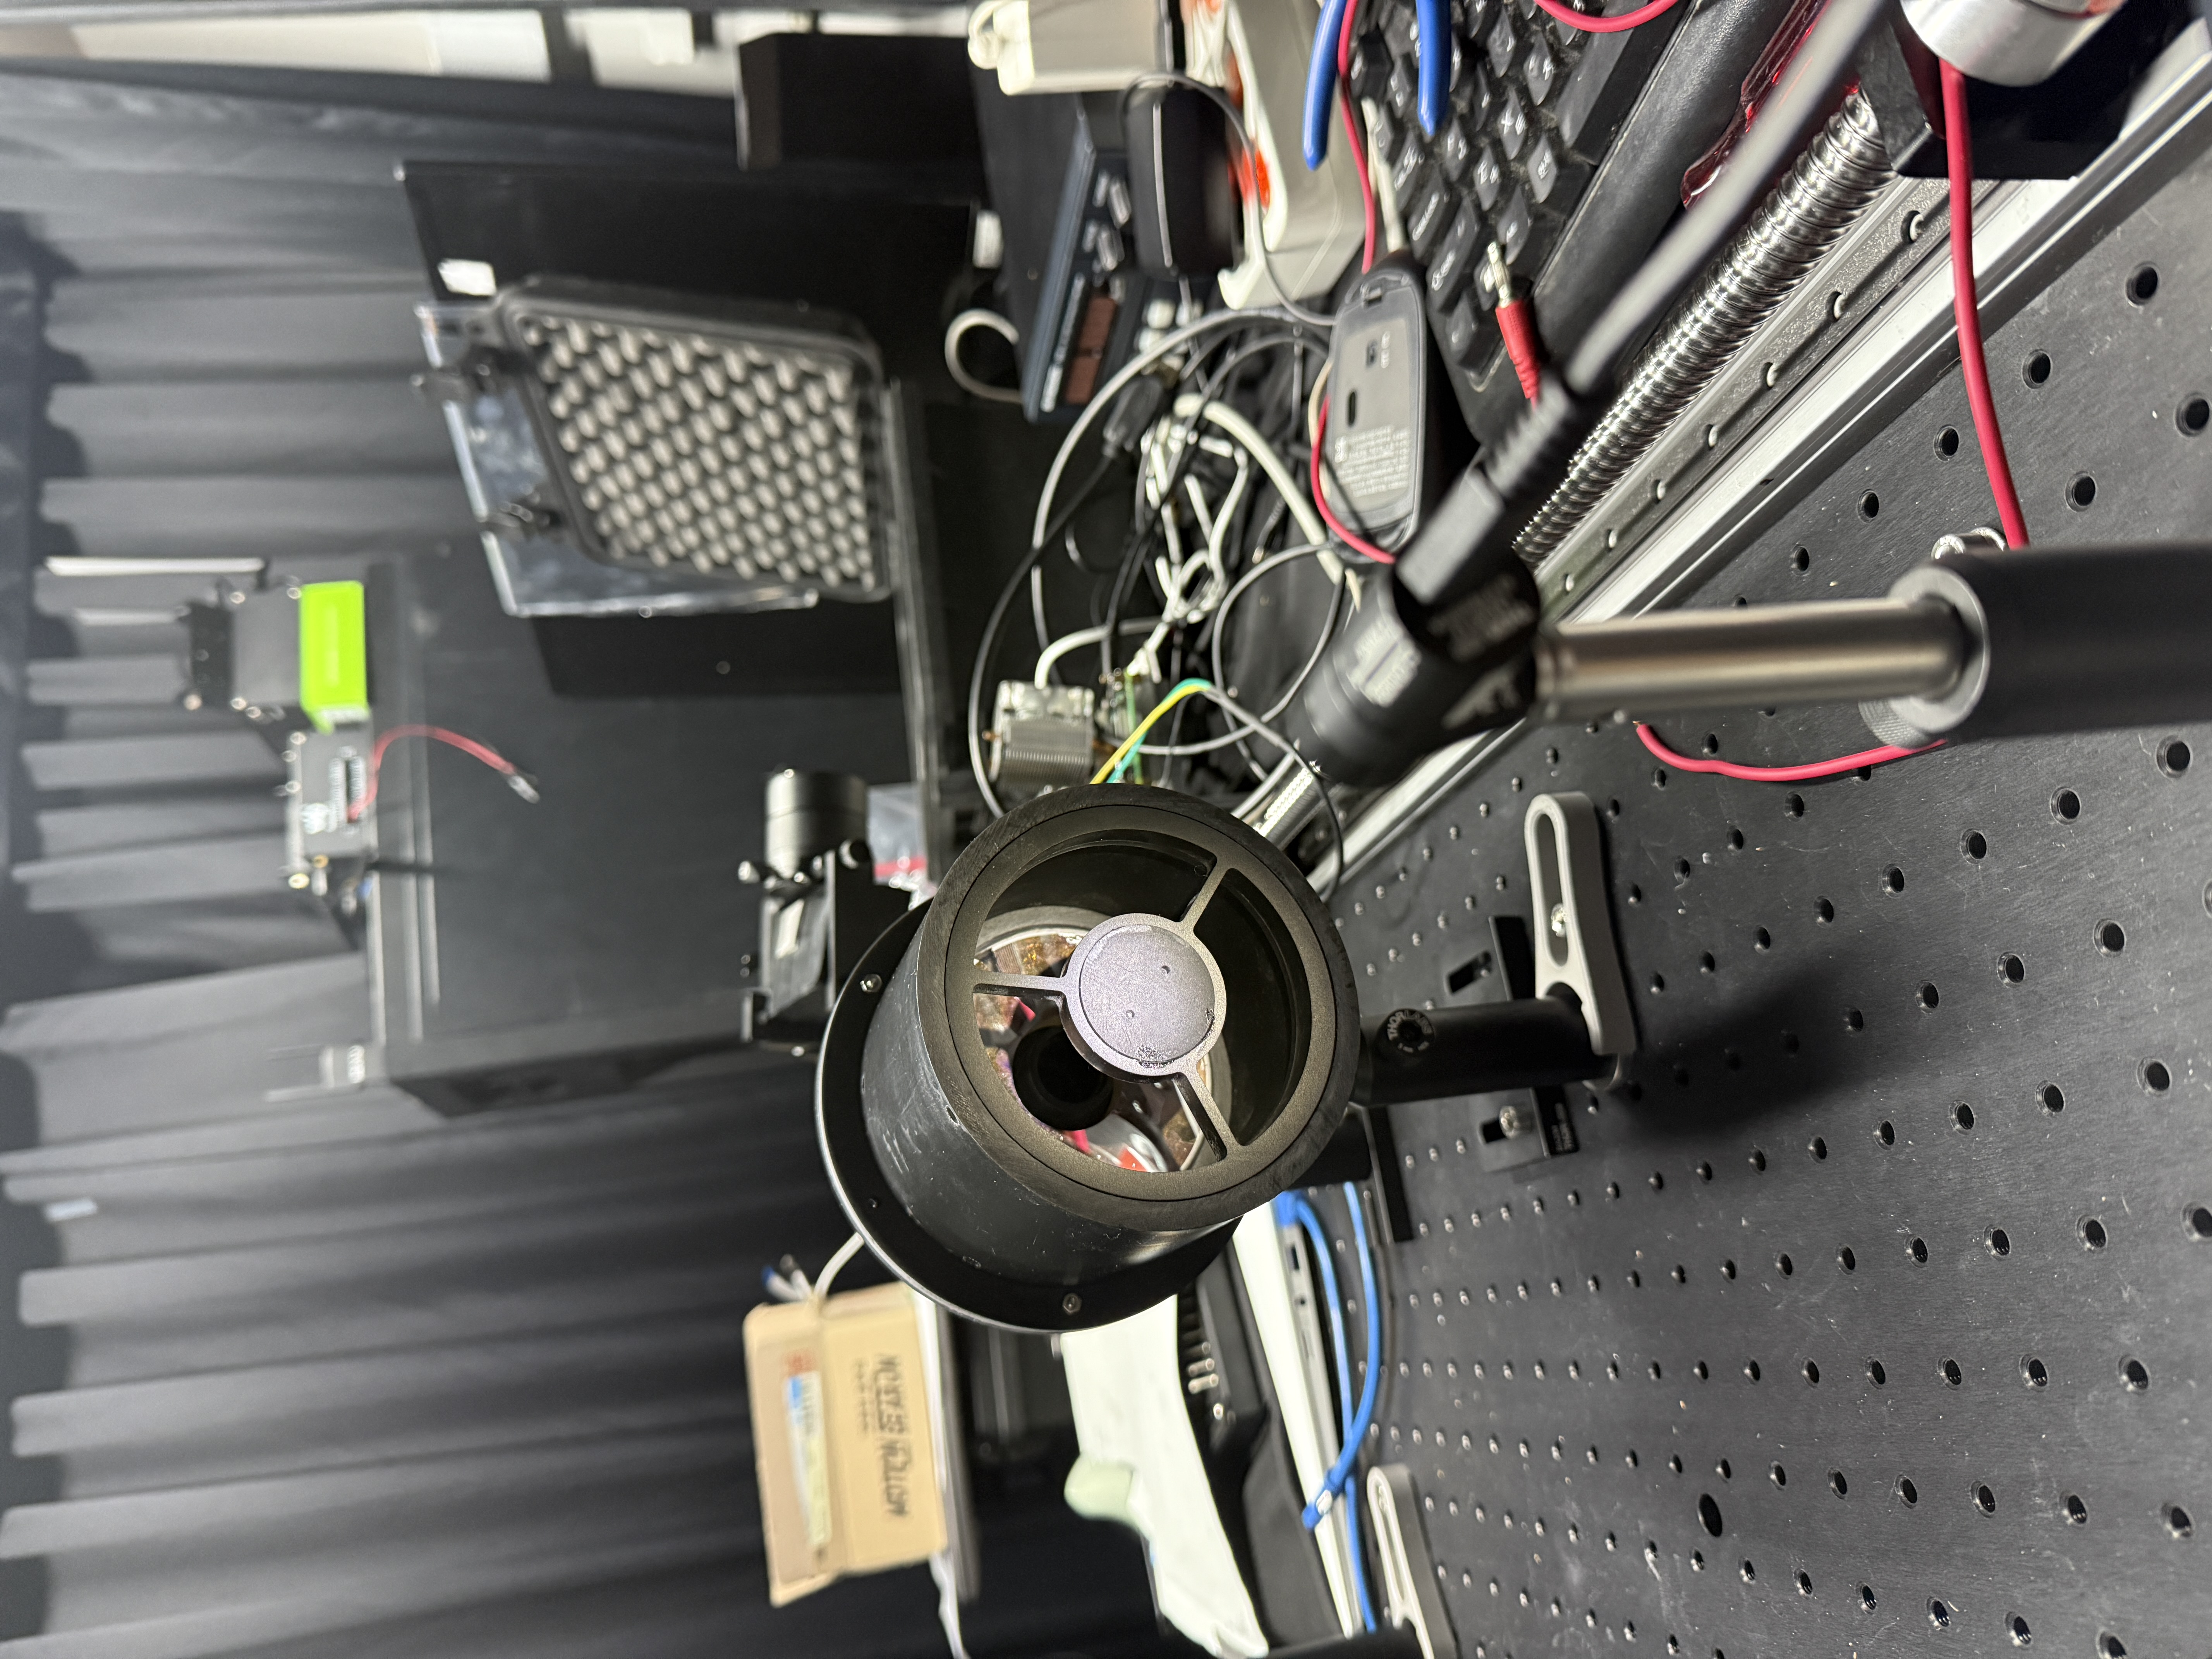
\includegraphics[width=45mm,angle=-90]{figs/Exp12.jpg}
		\caption{Initial experimental setup}
	\end{subfigure}
	\caption{Experimental configuration of assembled hyperspectral optical imager}
	\label{fig:expsetup}
\end{figure*}
The design trade space couple’s aperture, F-number, spectral coverage, MTF and SWaP. The internal-image plane modification enables a compact 118 mm optical track and 1.2U payload envelope, at the cost of a linear central obscuration of 0.48 and the requirement that residual aberrations of the fore-optic be absorbed by the collimator lens group. Both costs are acceptable for the target mission: the obscuration is compensated in the radiometric budget by the fast internal f/1.07 throughput and by the low-groove-density transmission grating, and the aberration absorption is achieved by joint re-optimisation of the collimator with the fore-optic. Compared with freeform CubeSat HSIs \cite{liu2021freeform}, the proposed design achieves comparable spatial and spectral resolution within a similar envelope while avoiding freeform manufacturing. Compared with Offner-type designs such as \cite{lee2008optical}, the on-axis prism–grating configuration trades off some spectral bandwidth for reduced alignment complexity and lower polarisation sensitivity. Compared with the in-orbit-demonstrated 1.5U TMA-based HSI of \cite{esposito2019inorbit}.
\section{Conclusion}
This paper presented a SWaP-optimised hyperspectral optical payload architecture for LEO precision-agriculture missions in a 3U CubeSat, together with the architectural description of an onboard AI data-reduction pipeline proposed for future integration. The optical design adopts a modified classical Cassegrain fore-optic in which the intermediate image plane is repositioned inside the primary–secondary envelope, coincident with the entrance slit of an on-axis prism–grating spectrometer. This modification, which adapts the embedded relay lens concept \cite{hsieh2011erlhis} to a spaceborne on-axis Cassegrain configuration, enables a total optical track of 118 mm and a payload envelope of 120×100×100 mm (0.4 at Nyquist, computed SNR of 78–120 across the 488-450nm range, and instrumental FWHM of 3.33 nm. The 8 W imaging power and 1.2U volume leave substantive SWaP margin within the 3U bus envelope for a co-located onboard AI accelerator, making the payload a suitable substrate for the proposed hybrid CNN Transformer selective-state space onboard segmentation architecture. End-to-end training and validation of the sensor and AI system are identified as the immediate future activity.
\section{Acknowledgements}
This research was supported by the Space-K BIG project program funded by the Korea Aerospace Administration (KASA) Grant No. RS-2025-16063273).
% Lists every entry of references.bib, including those not yet cited in the
% text. Delete this line before submission, once every source is cited, so
% that the reference list holds only works the paper actually cites.
\nocite{*}

\printbibliography

\end{document}
